\documentclass[12pt,a4paper]{article}

% Essential Packages
\usepackage{amsmath}
\usepackage{geometry} % Adjust margins
\geometry{margin=1in}
\usepackage{graphicx} % For images
\usepackage{fancyhdr} % Custom headers and footers
\usepackage{titlesec} % Custom section titles
\usepackage{hyperref} % Hyperlinks
\usepackage{xcolor} % Colored text and links
\renewcommand{\thesubsection}{\alph{subsection}}
\usepackage{listings}
\lstset{
  language=Python,
  frame=single,
  numbers=left,
  numberstyle=\tiny\color{gray},
  keywordstyle=\color{blue}\bfseries,
  stringstyle=\color{red},
  commentstyle=\color{green!50!black},
  basicstyle=\ttfamily\small,
  backgroundcolor=\color{gray!10},
  breaklines=true,
  showstringspaces=false,
  captionpos=b,
}

% Page Style


% Title Metadata
\title{Generative Transformers}
\author{Shaashvat Sekhar - WIDS 2k24}
\date{14 Feb 2025}

\begin{document}

\begin{titlepage}
    \centering
    \vspace*{1cm}
    {\Huge \textbf{Generative Transformers}}\\[1cm]
    {\Large Shaashvat Sekhar - WIDS 2k24}\\[1cm]
    {\large 14 Feb 2025}\\[1cm]
    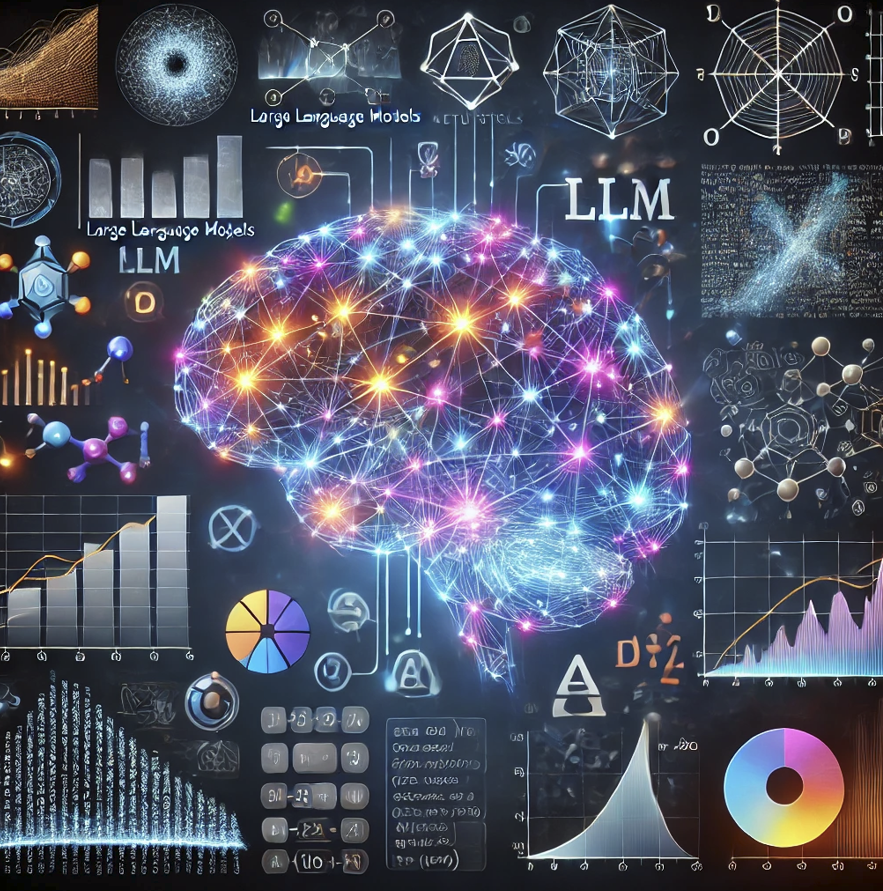
\includegraphics[width=1\textwidth]{cover}\\[1cm]
    \vfill
\end{titlepage}
\tableofcontents
%%% Intro
\pagebreak
\section{Introduction}
The link to my entire project can be found on GitHub \\

\url{https://github.com/shaashvats/Generative-AI-Transformer/tree/main/}
\subsection{Transformers}
Transformers have emerged as one of the most versatile and powerful architectures in modern machine learning, driving advances in natural language processing and generative AI. \\

Their ability to handle complex patterns and dependencies in data has made them foundational for large language models (LLMs) and other generative AI tools, which are rapidly shaping the future of technology and communication.\\
\subsection{Acknowledgments}
 \ \ \ \ \ My motivation to do this project was to learn the underlying maths of a transformer, and to learn how to implement a basic generative transformer.\\

I thank my mentors Aditya Neeraje, and Yash Sabale for giving me this opportunity, guiding me through this project, and providing useful resources. \\

I thank the Analytics Club IIT Bombay, and WiDS 4.0 for connecting me with my mentors. \\

Shaashvat Sekhar


\pagebreak


%%% Updates from lab 4
\section{Week One}
In the first part of the project I familiarised myself with some python libraries and tools, and implemented gradient descent
\subsection{Familiarization, and Insights}
\begin{itemize}
\item Python is a relatively easy language to write code in because it is a high-level language with english-like syntax and has lots of useful libraries for ML
\item NumPy has a feature called broadcasting which enables simultaneous element-wise operation on arrays of different shapes using vectorization. It enables fast matrix operations, making it useful for ML
\item Jupyter Notebooks are useful for creating projects because they have blocks which can be used to write and execute code systematically one step-at-a-time. They are also compatible with with LaTeX for equations, MatPlot Lib for visualising and all other python libraries
\end{itemize}

\subsection{Gradient Descent}
\begin{itemize}
\item Gradient Descent is a method to find a local minima of a continuous function. It is based on the principles of multivariable calculus, and concepts of partial derivatives and gradient.
\item The greatest descent of a function at a point $x$ is in the direction of: $-\nabla f$
\item By iteration of:
 \[x_{i+1} = x - \alpha * \nabla f(x_{i})\]
\subitem Where $\alpha$ is called the "learning rate" and is a small positive constant, we can find a local minima of a functions (with some limitations)
\item $\alpha$ Can be dynamic to do gradient descent in less iterations (epochs). The "adam" optimizer uses this idea.
\item I used gradient descent to find a local minima of 
\[f(x) = x^4 + x^2y^2 - y^2 + y^4 + 6 \]
\item This function has two local minimas, and gradient descent based on the initial position, ends up at (0, -7.07) or (0, 0.707)
\item This demonstrates that gradient descent can be used to find a local minima but not necesserily a global minima 
\item (code, outputs, visualisation: on next page)
\pagebreak
\begin{figure}[h!]
    \centering
    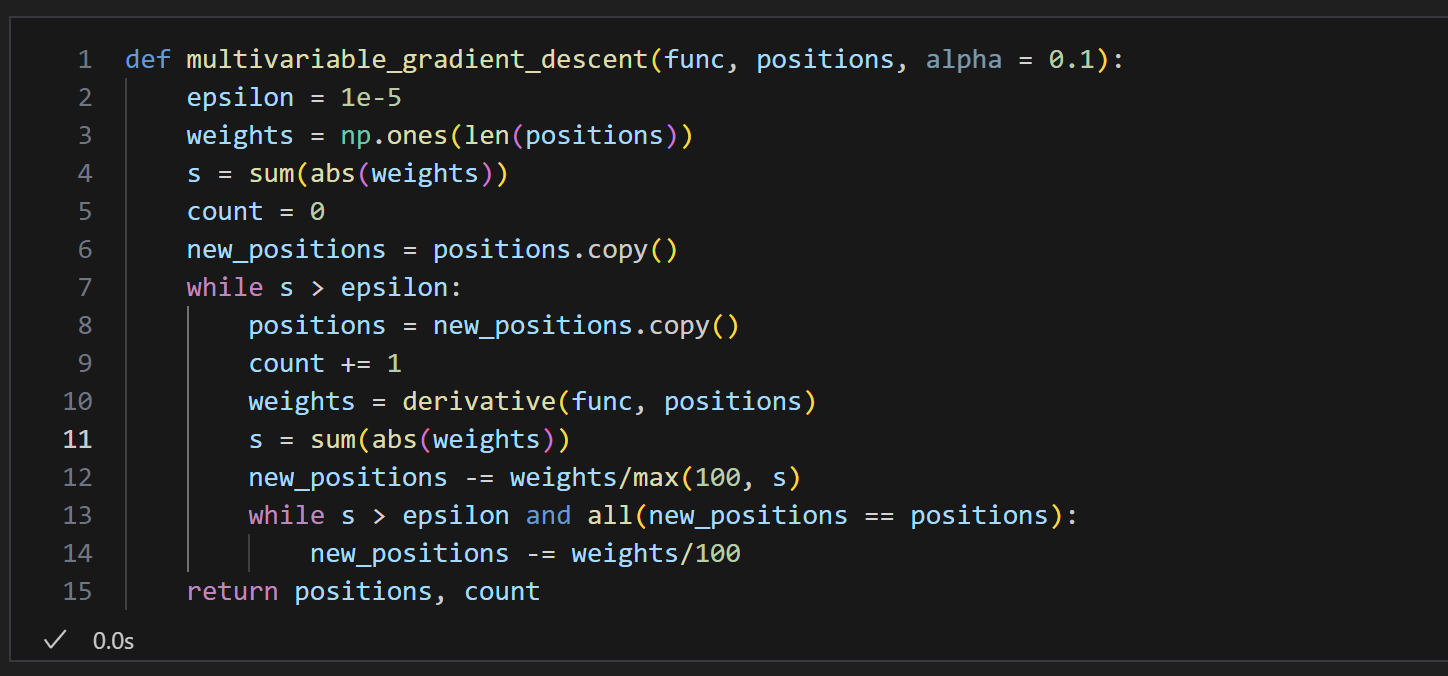
\includegraphics[width=0.8\textwidth]{grad1} 
    \caption{Gradient Descent Algo}
    \label{fig:example}
\end{figure}

\begin{figure}[h!]
    \centering
    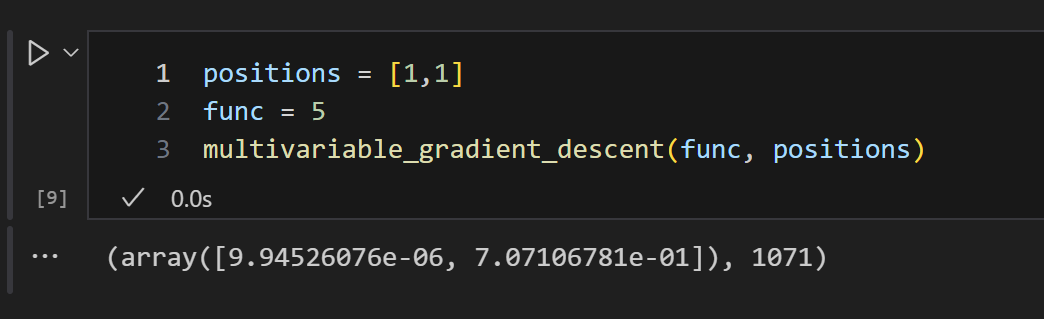
\includegraphics[width=0.8\textwidth]{grad2} 
    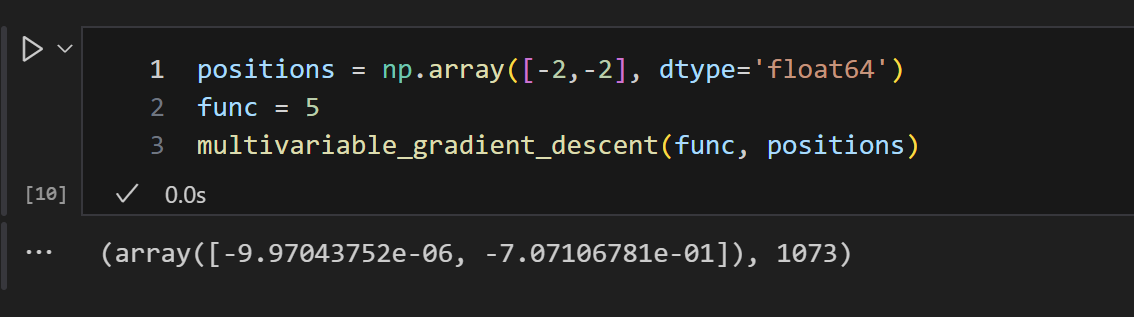
\includegraphics[width=0.8\textwidth]{grad3} 
    \caption{Gradient Descent Output}
    \label{fig:example}
\end{figure}
\begin{figure}[h!]
    \centering
    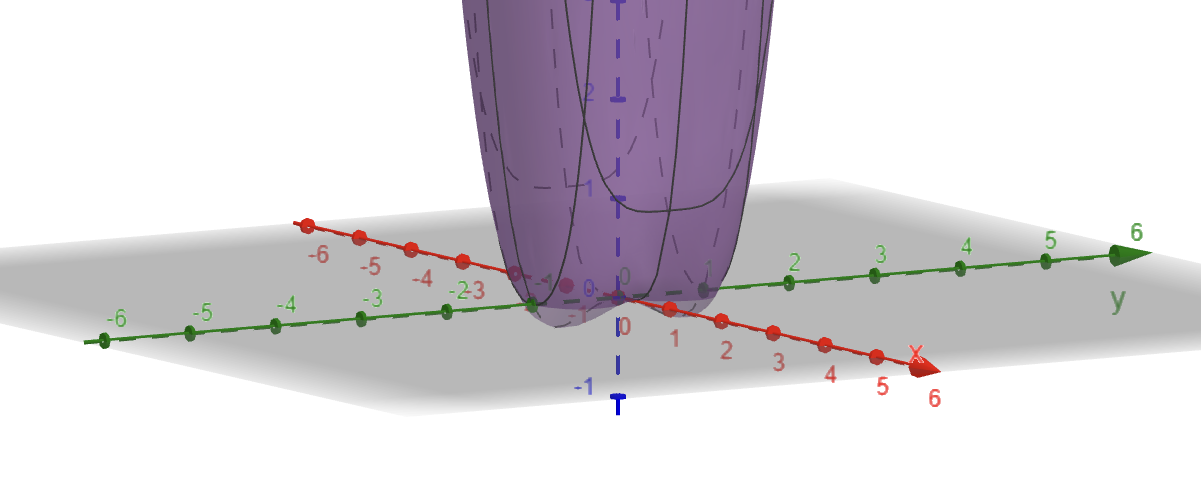
\includegraphics[width=0.8\textwidth]{grad4}
    \caption{Function Visualisation}
    \label{fig:example}
\end{figure}
\end{itemize}
\pagebreak
%%%%%%% WEEK 2
\section{Week Two}
In week two, I learned theory behind feedforward neural networks and used it to implement simple neural networks carrying out Boolean operations of two inputs
\subsection{Feedforward Neural Network}
\begin{itemize}
\item A feedforward neural network has multiple layers of "neurons" $A^{(i)}$
\item Each layer of neurons is created by a linear combination of the previous layer (inputs for layer-1) plus addition of bias, and finally a passthrough a non-linear activation function $ \sigma$. This process is called \textbf{Forward Propogation.}
% Weighted Sum and Bias (Hidden Layer)
\[ z^{(1)} = W^{(1)}x + b^{(1)} \]
% Activation Function (Hidden Layer)
\[ a^{(1)} = \sigma(z^{(1)}) = \sigma(W^{(1)}x + b^{(1)}) \]
% Output Layer
\[ z^{(2)} = W^{(2)}a^{(1)} + b^{(2)} \]
% Output Layer Activation (e.g., Softmax)
\[ \hat{y} = \sigma_{\text{out}}(z^{(2)}) \]
\item Each neuron acts like a logistic regression. Having multiple neurons allows the model to "learn" different patterns. The "knowledge" is stored in the coefficients and biases which can create interesting effects because of the non-linear activation
\item The generalised expression:
% Matrix Form for Multiple Layers
\[ a^{(l)} = \sigma(W^{(l)}a^{(l-1)} + b^{(l)}), \quad \text{for } l = 2, 3, \dots, L \]
\[ a^{(0)} = x \quad \text{(input layer)}, \quad a^{(L)} = \hat{y} \quad \text{(output)} \]
\item Loss is calculated through Binary Cross Entropy, and the sum of the loss across several test cases is used to determine how coefficients and biases are to be updated to improve the models functioning
% Loss Functions
% Cross-Entropy Loss for Classification
\[ \mathcal{L} = -\sum_{i=1}^{N} y_i \log(\hat{y}_i) \]
\item We differenciate the loss with respect to the coefficients of different layers and update the coefficients based on the gradient. .We do not find the "exact" gradient with respect to all coefficients at once, rather,  we go layer by layer and iterate each layer independantly. This process is called \textbf{Backward Propogation.} and it is used to make the model "learn"
% Backpropagation (Gradient Calculation)
\[ \frac{\partial \mathcal{L}}{\partial W^{(l)}} = \frac{\partial \mathcal{L}}{\partial a^{(l)}} \cdot \frac{\partial a^{(l)}}{\partial z^{(l)}} \cdot \frac{\partial z^{(l)}}{\partial W^{(l)}} \]
% Weight Update Rule (Gradient Descent)
\[ W^{(l)} := W^{(l)} - \eta \frac{\partial \mathcal{L}}{\partial W^{(l)}} \quad,\quad b^{(l)} := b^{(l)} - \eta \frac{\partial \mathcal{L}}{\partial b^{(l)}} \]
\item The inital coefficients and biases are set randomly in a process known as \textbf{Seeding}. They are set randomly instead of uniformly because of the way back propogation works, symmetric weights would make the model not learn diverse traits, rather, it would behave very primitively. 
\end{itemize}
\subsection{Hyperparameter Tuning}
\begin{itemize}
\item Hyperparameter tuning is done during the training of a machine learning model to find the best settings that improve how well the model learns before testing it on new data.
\item It helps the model work better by avoiding mistakes like underfitting (too simple) or overfitting (too complex), and affecting how quickly the model learns
\item What can be tuned:
\subitem Learning Rate ($\eta$) determines how quickly the model changes coefficients and biases. A higher $\eta$ can find a minima quicker, with a risk of overshooting.
\subitem Number of Epochs determines how many iterations of the model are done. Too many can create overfitting, too few can create underfitting
\subitem Activation function determines how loss is calculated and how the model behaves. If affects how the model learns, and the nature of outputs it can generate
\item For the simple AND, XOR, Full-Adder Neural networks, hyperparameter tuning was not important because of how trivially the network was required to behave. However, for The Boston Housing Data, I did use it to improve model predictions
\end{itemize}

\subsection{Perceptron} 
\begin{itemize}
\item A perceptron is the simplest configuration of a feedforward neural net. It has no hidden layer. It has n inputs, one output, and only one activation. \\
\[ z^{(1)} = W^{(1)}x + b^{(1)} \]
\[ f(x) = h( z^{(1)}) \]
\[\text{h(u) is the Heaviside function where} \\  \  h(u) = 1 \ \forall \ u \ \ge 1, h(u) = 0 \ \ \text{o.w.} \]
\item I made a slight change: I used the sigmoid activation instead of h(u). This allowed me to use binary cross entropy to calculate loss, and use the related formulas for backpropogation on g(x). 
\[ g(x) = \sigma( z^{(1)}) \]
\item I then rounded the outputs to get f(x), my output.
\[ f(x) = \text{Round}(\sigma( z^{(1)})) \]
\item The general idea of how a sigmoid activation works is that Z is a linear combination of inputs, and the sigmoid activation is a monotonically increasing function with a sharp rise from 0 to 1 around origin. This means that a sigmoid activation works like a classifier of a linear combination of inputs.
\begin{figure}[h!]
    \centering
    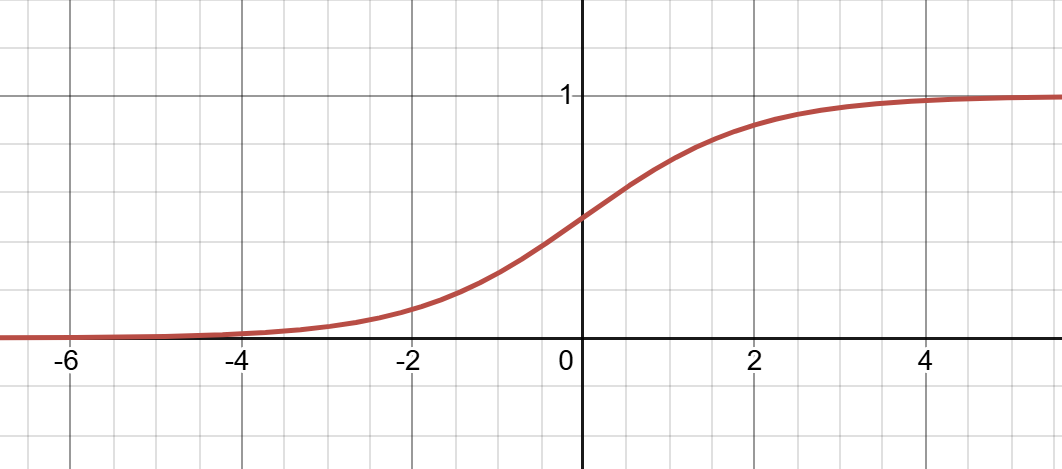
\includegraphics[width=0.7\textwidth]{sigmoid} 
    \caption{Sigmoid Function}
    \label{fig:example}
\end{figure}
\item For AND: This would work along the following lines:
\subitem The output  $y = a\land b$ is 1 only when a=1 and b=1. In all other cases, the output y = 0. We can see a clear linear demarcation of y on the basis of a+b where $y =1 \iff a+b > 1 $  
\subitem We exploit this by using coefficients, bias: $ z = \beta *(a+b -1.5) $  
\subitem Which ensures  $z$ would be positive only when both $a=1$ and $b=1$ and otherwise it would be negative. 
\subitem A sufficiently large $\beta$ would move $z$ far enough from the origin that the output of the sigmoid activation would be very close to 0 when $z<0$ and very close to 1 when $z>0$. Thus a perceptron can very easily model an AND gate.
\item For XOR: There is no linear combination of a,b that can demarcate (0,1) and (1,0) from (1,1) and (0,0). Hence a perceptron cannot model an XOR Gate



\end{itemize}

\subsection{Perceptron Implementation of AND}
\begin{itemize}

\item I used sigmoid activation for backpropogation and then rounded to get results 
\subitem (see code in Week 2 of project)
\item The final weights and bias came to be similar to what I had expected
\subitem (see previous section)
\item \textbf{XOR} \ The perceptron model couldn't model XOR gate as expected
\end{itemize}
\begin{figure}[h!]
    \centering
    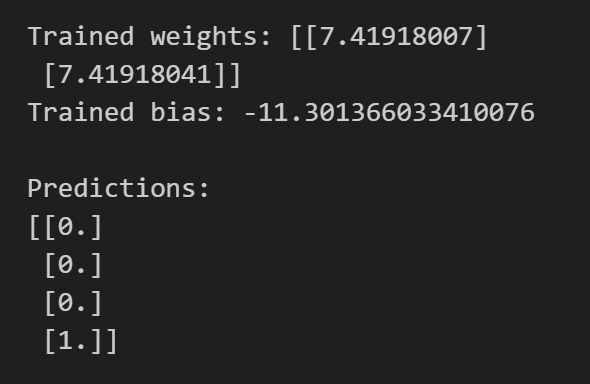
\includegraphics[width=0.4\textwidth]{AND} 
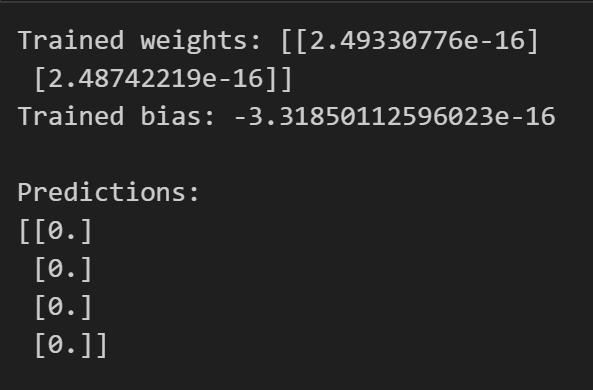
\includegraphics[width=0.4\textwidth]{XOR_fail} 
    \caption{Successful AND (Left) - Unsuccessful XOR (right)}
    \label{fig:example}
\end{figure}
%%% \begin{lstlisting}
%%%% \end{lstlisting}
\subsection{Neural Net Implementation of XOR}
\begin{itemize}
\item I used a neural net with one hidden layer. The hidden layer had two neurons.
\item I rewrote the functions for forward propogation and backward propogation to account for the additional hidden layer item. The neural net was successfully.
\item The intuition here is that (1,0) can be demarcated from the other 3 inputs and so can (0,1). One of the hidden neurons activates only for the prior and the other, for the latter. The output neuron then activates if atleast one of the hidden neurons does. The inference drawn here is that non convex behaviour can be modelled by many convex activations, something which one convex non-linear activation cannot do
\end{itemize}
\begin{figure}[h!]
    \centering
    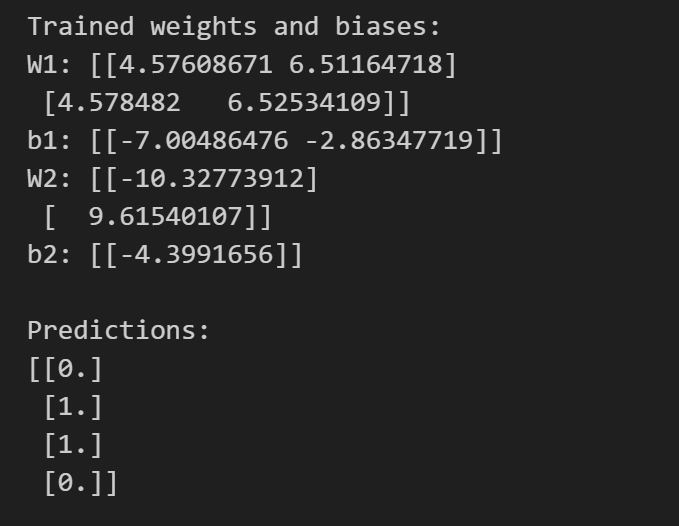
\includegraphics[width=0.4\textwidth]{XOR_succ} 
    \caption{Successful XOR using 2 Hidden Layer Neurons}
    \label{fig:example}
\end{figure}
\subsection{Neural Net Implementation of Full Adder}
\begin{itemize}
\item In this case, two hidden neurons were insufficient but three were sufficient. 
\item Note: there are two outputs for a full adder, as opposed to one
\item It seems obvious to me that the full adder requires more hidden neurons to "learn" more complex behaviour. However I couldn't predict for a more complicated circuit, or why its 3 and not 4 here.
\end{itemize}
\begin{figure}[h!]
    \centering
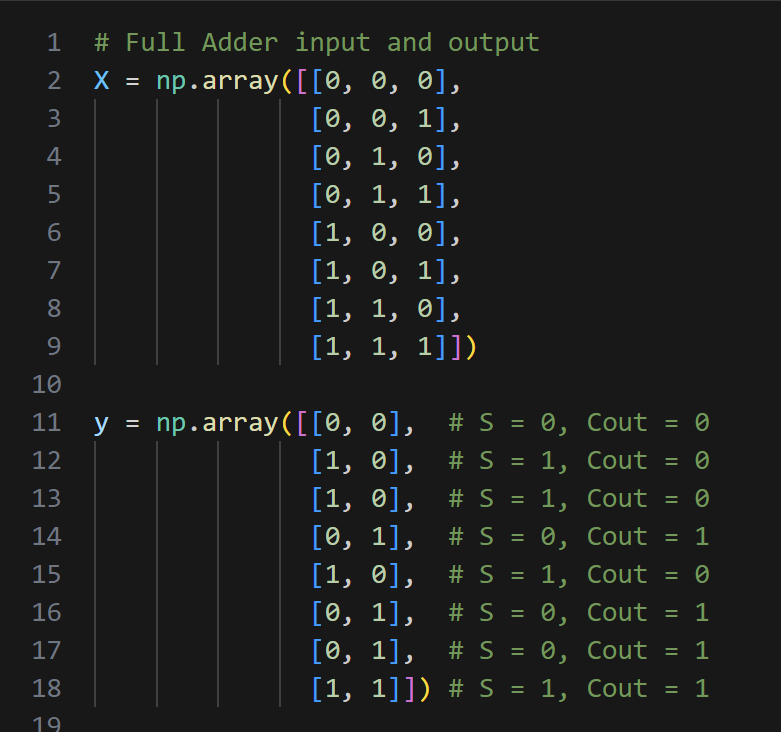
\includegraphics[width=0.4\textwidth]{full_in} 
    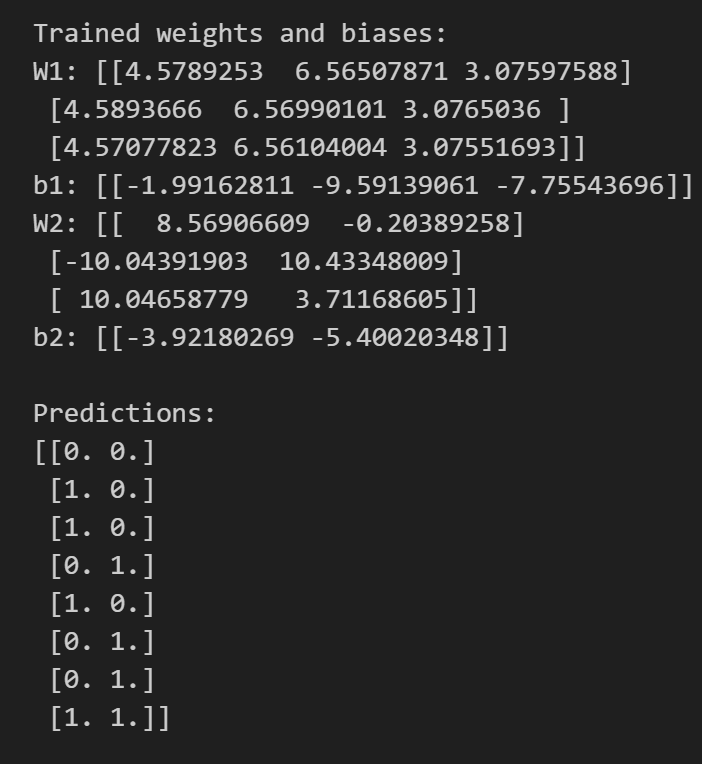
\includegraphics[width=0.4\textwidth]{full} 
    \caption{Full Adder Training Data (left), Model (right)}
    \label{fig:example}
\end{figure}
\pagebreak
\subsection{Ripple Carry Adder}
\begin{itemize}
\item For the Ripple carry adder, I did multiple feedforwards using the Full Adder neural net coefficients I obtained. I cascaded the process to feed the computed carry-out of the n-th addition to the carry-in of the (n+1)-th
\end{itemize}
\begin{figure}[h!]
    \centering
    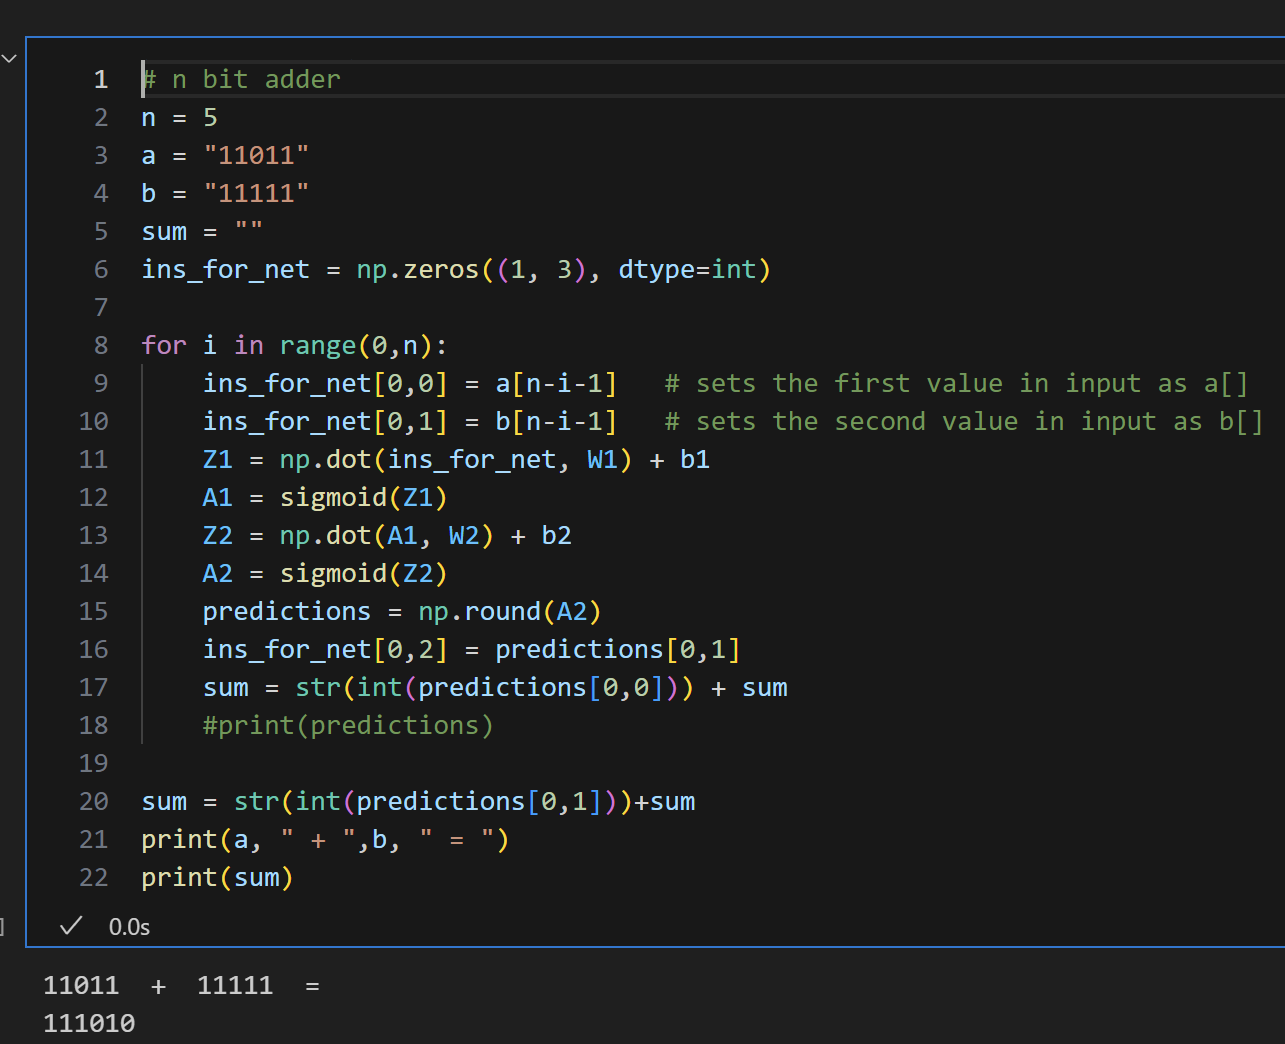
\includegraphics[width=0.8\textwidth]{ripple} 
    \caption{Ripple Carry Adder}
    \label{fig:example}
\end{figure}
\pagebreak
\section{Week Three}
I implemented a neural net to predict house prices in the well-known Boston Housing Dataset. I learnt to improve, and gauge model performance by tuning hyperparameters.
\begin{lstlisting}
Number_of_train = 300
np.random.shuffle(data)
x_train = data[0:Number_of_train, :-1]
y_train = data[0:Number_of_train, -1]
x_test = data[Number_of_train:, :-1]
y_test = data[Number_of_train:, -1]
model = tf.keras.Sequential([
    tf.keras.layers.Dense(40, input_dim=13, activation='relu', use_bias=True),
    tf.keras.layers.Dense(40, activation='relu', use_bias=True),
    tf.keras.layers.Dense(1)  
model.compile(optimizer='adam', loss='mean_squared_error')
model.fit(x_train, y_train, epochs=100, batch_size=300)
test_loss = model.evaluate(x_test, y_test)
y_pred = model.predict(x_test)
\end{lstlisting}
\subsection{Preprocessing}
\begin{itemize}
\item I shuffled the data to ensure that the order in which data was collected did not affect which data was used to train the model and which would be used to test.
\item I trained the model on 300 instances, and used the rest $\approx$ 200 to test. 

\end{itemize}
\subsection{Model}
\begin{itemize}
\item I changed different parameters till I could get a model that had really low loss, and had a similar loss on the train data as the test data. This was to neither overfit, nor underfit the model onto the data.
\item This brought an interesting question to my mind: Given a training dataset, how well can we theoretically make predictions using a neural net on a test dataset?
\item I used a high number of epochs for the model. This allowed the model to go very close to ideal behaviour. I lost count of the total number of epochs I used.
\item A small batch size has a faster epoch time, but creates noisier updates. I tried using a combination of both small and large batch sizes. Given the size of the data, it didn't matter which batch size I used to save time, but an insight I drew into training larger models is that we can initially use small batch sizes to get close to a minima, and use a large batch sizes for fine-tuning the model as we get closer.
\item I used relu as the activation function. I did this because the outputs were unbounded, and of an analog nature rather than a yes-no bounded nature. Sigmoid and tanh didn't work as they can't handle the range of values that a linear/polynomial function requires, that I tried to model prices as. Similarly, I used mean-square error to calculate loss.
\item I used two hidden layers, each of 40 neurons. My intuition suggested that the model can learn traits in line with the minimum number of neurons it has in a layer. So when I created multiple layers I thought it would be best to have equal number of neurons in each layer. With fewer layers, the model had some instances with very large loss. This suggested that the model didn't have enough neurons to account for that pattern of behaviour. Increasing the number of neurons solved this issue.
%\begin{lstlisting}
%\end{lstlisting}
\begin{figure}[h!]
    \centering
    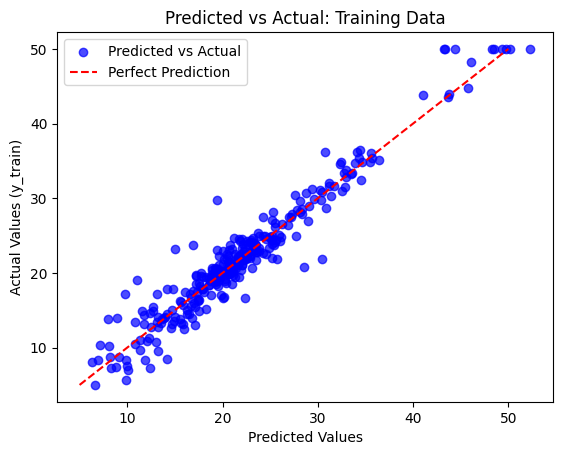
\includegraphics[width=0.7\textwidth]{3_train_img} 
    \caption{Model performance on training data}
    \label{fig:example}
\end{figure}
\begin{figure}[h!]
    \centering
    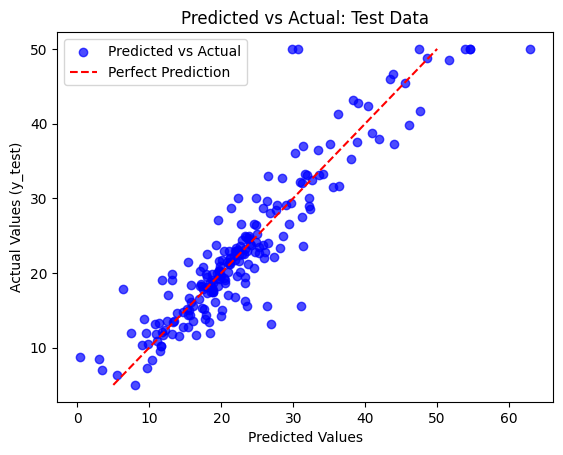
\includegraphics[width=0.7\textwidth]{3_test_img} 
    \caption{Model performance on test data}
    \label{fig:example}
\end{figure}

\subsection{Some Failures}
\item Tanh/Sigmoid in both layer activation couldn't model linear/polyonmial behaviour
\begin{figure}[h!]
    \centering
    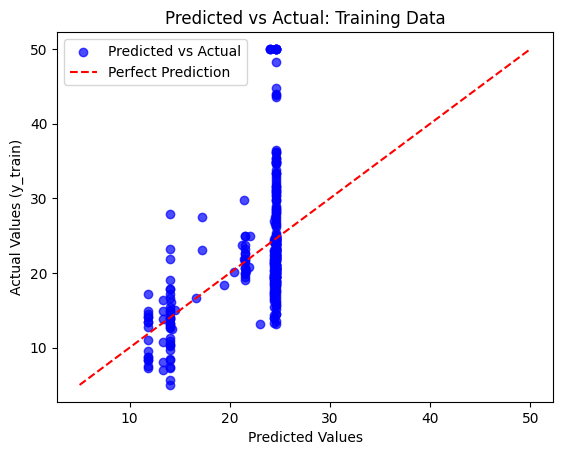
\includegraphics[width=0.45\textwidth]{3_tanh} 
    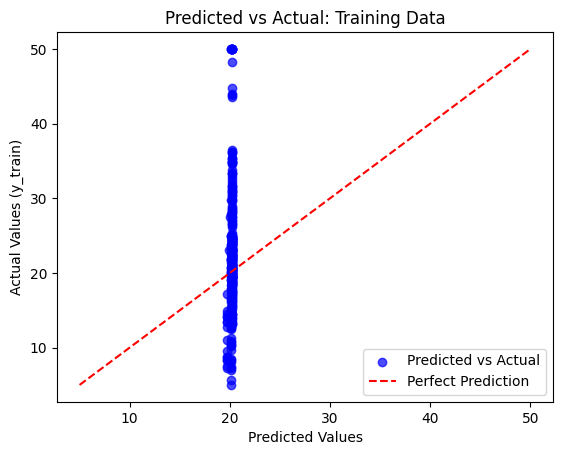
\includegraphics[width=0.45\textwidth]{3_sigmoid} 
    \caption{Tanh (left) - Sigmoid (right)}
    \label{fig:example}
\end{figure}
\item Using a combination of tanh, relu couldn't model linear/polyonmial behaviour
\begin{figure}[h!]
    \centering
    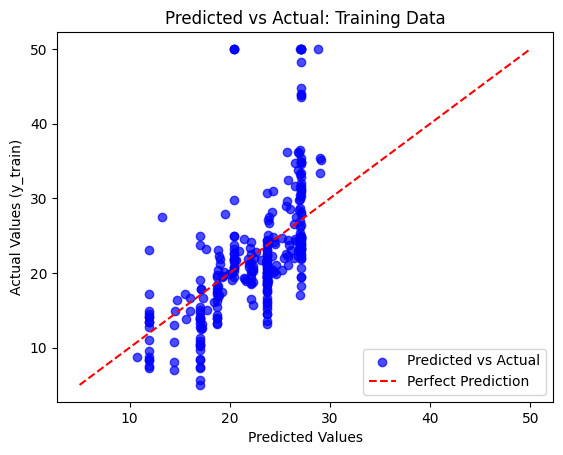
\includegraphics[width=0.45\textwidth]{3_tanh_relu} 
    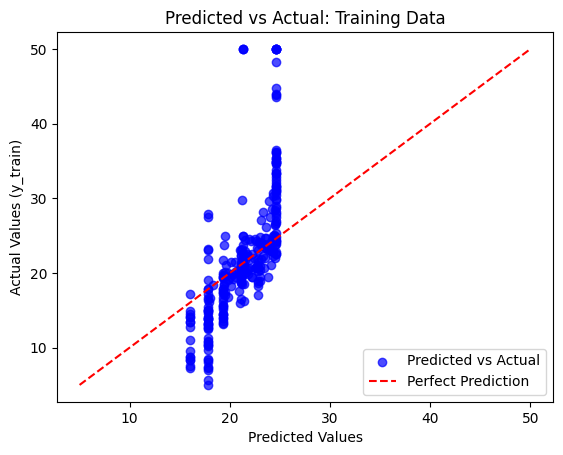
\includegraphics[width=0.45\textwidth]{3_relu_tanh} 
    \caption{Tanh then Relu (left) - Relu then Tanh (right)}
    \label{fig:example}
\end{figure}
\end{itemize}
\pagebreak
\section{Week Four}
In week four, I learnt the theory behind the architecture of transformers and implemented one to produce text like Shakespeare using generative character prediction. 
\subsection{Transformer Theory}
\begin{itemize}
\item \textbf{Tokenization} converts words to tokens, making a string a series of tokens
\item \textbf{Token Embedding} assigns each token a vector in a high dimension space which begins to hold information of the meaning of the word
\item \textbf{Positional Encoding} assings each position before the next word a vector in the same space as token embeddings
\item \textbf{Attention} updates embeddings of latter embeddings based on their previous embeddings using Query, Key, and Value. Attention block helps the model learn context and how one word affects another after it.
\item \textbf{Neural Net} predicts the next embedding based on the N embedding output of the attention block
\item \textbf{Decoder}, finally, predicts the next word based on the embedding output of the neural net using softmax
\item The oldest word is removed, the other words are shifted and the new word is added to the string. The new string is fed to the transformer and it agains repeats the process of predicting the next word.
\item The transformer is trained similar to a neural network, using Backpropogation 
\end{itemize}
\subsection{Character Tokenization}
\begin{itemize}
\item In my first attempt at building a Large Language Model (LLM), I tokenized the characters not the words
\item Given the sparse nature of training data, and very few epochs of training implemented, this resulted in some illegible text output (See next page)
\item In some sense, it is a successful "stochastic parrot" because it is generating new tokens, however this is not what I had set out to achieve. 
\item Something I learnt from this endeavour is that LLMs take a lot of compute to train. This primitive one took ten hours for ten epochs. 
\item (Unofficial conclusion) I did not have the motivation to build the correct version of the Shakespeare parrot (where I tokenize words instead). This leaves me feeling a slight lack of closure, which I hope to channel some of into building more technical, detailed projects involving ai/ml/transformers/llms in the future. I hope that the efforts I have put into this project reflect a growing understanding of AI and my eagerness to learn.
\end{itemize}
\pagebreak
\begin{figure}[h]
    \centering
    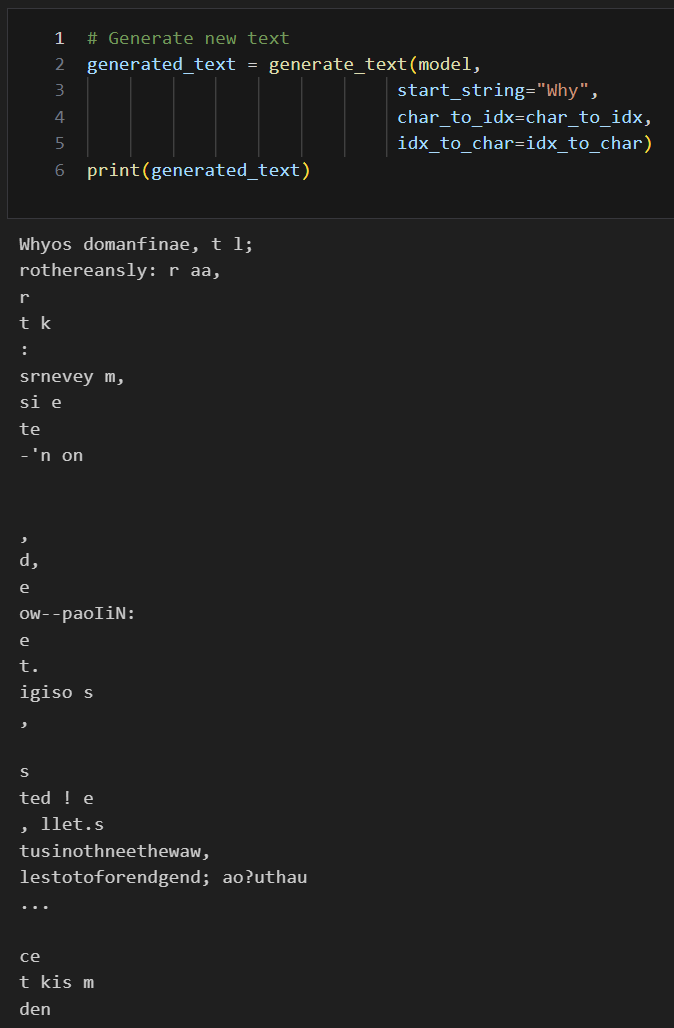
\includegraphics[width=0.7\textwidth]{gen_1} 
    \caption{Character tokenization}
    \label{fig:example}
\end{figure}
\pagebreak
\section{Conclusion}
This is the first project in machine learning that I have completed. Over the course of the project, I have learned to work with TensorFlow, Keras, and NumPy, using them to implement various machine learning models. In weeks one and two, I implemented perceptrons and neural networks to model logical gates.
In week three, I developed a neural network to predict house prices using the Boston housing dataset with TensorFlow. Finally, I implemented a transformer model for character generation, training it on Shakespeare's texts.

By building these models, I have gained a solid foundation in machine learning and artificial intelligence. Familiarizing myself with the transformer architecture has helped me understand its applications in various generative AI systems.  This project has sparked my interest in exploring the theoretical foundations of artificial intelligence and in creating projects that leverage it to generate value for society.

\section{Bibliography, References}
\begin{itemize}
\item \url{https://github.com/AdityaNeeraje/Generative-AI-Transformer}  \\ by Aditya Neeraje and Yash Sabale
\item Stanford CS229: Machine Learning, by Andrew Ng
\item Deep learning Video Series, by 3b1b on YouTube
\item ChatGPT and Claude.ai: for code and report-writing
\item Boston Housing Data, by US Census Service
\item Shakespeare's work, by Shakespeare
\end{itemize}


\end{document}

